% !TEX encoding = UTF-8
% !TEX TS-program = pdflatex
% !TEX root = ../tesi.tex

%**************************************************************
\chapter{State of the art}
\label{cap:state-of-the-art}
\intro{This chapter discusses the \textbf{state-of-the-art} in relation to the scope this project, with a coverage of multiple topics which constitute the background of our work.}

\section{An overview on Game Engines}
\intro{In this section we discuss the main features of Game Engines, with an overview of Legacy Game Engines and their shortcomings.}
\subsection{Definitions}
Game Engines (GEs) are generally defined as software frameworks designed for the development and execution of interactive multimedia software, namely video games. \\
More specifically, we define video games a the subset of games that take place in a 2-3 dimensional virtual world, with a variable number of players \cite{womak:distributed-cloud-gaming-pipeline}. Considering that:
\begin{itemize}
	\item the world where they take place is time dependant (temporal or dynamic);
	\item the time in the simulated world is a mathematical approximation and simplification of reality;
	\item there are multiple distinct entities known as "agents" that interact in this world;
\end{itemize}
video games can be seen as \textit{soft-time interactive agent-based temporal computer simulations}, where the interaction of an user with an interface or input device provides them with a visual feedback \cite{site:game-engine-wiki, womak:gregory-game-engine}. \\ \\
If we look at them on the surface level, it might be hard to differentiate Game Engines from video games software. \\
In this context, according to Jason Gregory in his book "Game Engine Architecture" \cite{womak:gregory-game-engine}, the main characteristic that defines a Game Engine is its \textit{data-driven architecture}.
Video games software usually contains hard-coded logic or game rules, to manage their functionalities through non-reusable code. On the other hand, Game Engines aim towards the possibility of creating multiple products with new elements and functionalities, through minimal changes performed to the original "engine" software. \\ \\
As such, we can define a Game Engine as a \textit{piece of software that is extensible and can be used as the foundation for many different video games without major modifications} \cite{womak:gregory-game-engine}. \\ \\
\begin{figure}
	\centering
	\includegraphics[width=1\linewidth]{"immagini/State-of-the-art/Reusability gamut"}
	\caption[Game engine reusability gamut - Gregory]{Game engine reusability gamut - Gregory.}
	\label{fig:reusability-gamut}
\end{figure}

\subsection{Structure}
As we discussed in the previous section, reusability is the most paramount characteristic of Game Engines. As such, Game Engines cannot be composed just of libraries and tools for merging multimedia assets \cite{womak:revamping-cloud-games}. A portion of Game Engine software needs to become a part of the developed video game itself, with the purpose of managing these reusable functionalities. \\ \\
For this reason, Game Engines generally consists of two main components:
\begin{itemize}
	\item a \textbf{tool suite}, which allows non-technical users to create and manage audiovisual assets, such as: 3D meshes, textures, sounds and animations. This component is left behind after the game development process, since it is not useful while playing \cite{womak:distributed-cloud-gaming-pipeline};
	\item a \textbf{runtime component}, which is transferred into the game executable in order to manage resources, schedule events and implement complex functionalities (e.g. 2D-3D graphics rendering, physics management, collision detection) that are reusable across multiple video games \cite{womak:gregory-game-engine, womak:revamping-cloud-games}.
\end{itemize}
The runtime component, in particular, is structured in multiple layers with an increasing level of abstraction. \cite{womak:revamping-cloud-games} \\ \\
As we can see in Figure \ref{fig:runtime-component}, the lowest level acts as an interface to the kernel and the hardware the game is running on. This is especially important for the implementation of core video game functionalities, such as graphics rendering and physics simulation, which heavily rely on the processing performed by the physical hardware (e.g. CPU, GPU, memory). \\ \\
On the other hand, the upper layers focus on providing an entry point for the game APIs, a certain degree of platform independence and game specific functionalities (e.g. AI, player mechanics, game cameras and online multiplayer capabilities).
\begin{figure}
	\centering
	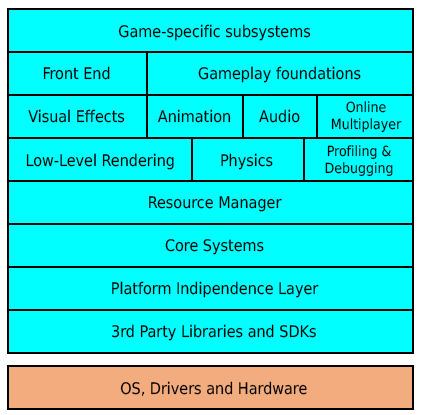
\includegraphics[width=0.60\linewidth]{immagini/State-of-the-art/runtime-component.png}
	\caption[Simplified layered structure of the runtime component.]{Simplified layered structure of the runtime component.}
	\label{fig:runtime-component}
\end{figure}

\subsection{Shortcomings of a monolithic architecture}
Even if many Game Engines are carefully crafted and fine-tuned to run particular games on specific hardware platforms \cite{womak:gregory-game-engine}, in most of them the core original \textbf{monolithic architectural model} is still present. \\ \\
As we discussed in the previous section, each instance of video game executable needs to embed the runtime component of the Game Engine used to develop it. This component runs alongside the main game instance, managing its core functionalities and thus creating an high degree of dependence on it. \\ \\
Game Engines implementing such monolithic architecture, which we will call \textit{Legacy Game Engines}, present three major shortcoming \cite{womak:revamping-cloud-games}:
\begin{enumerate}
	\item first, while providing high performance, a monolithic software requires refactoring of the whole project (or large part of it) at every change in the codebase. This operation can become quite expensive in the long run and turn into a production bottleneck, especially in context where changes are frequent;
	\item second, monolithic software operations processing can hardly be split among different server, as such we often run the risk of putting an excessive amount of CPU workload on a single centralized server. In this context, when resources are insufficient the centralized server becomes a bottleneck, significantly reducing the performance of the system. Moreover, this kind of services are hard to scale, since their only option is to vertically increase the quantity of resources available, in case of necessity. So, considering the online multiplayer scalability requirements of most recent video games, which connect up to even hundreds of players \cite{site:mmo-wiki} to the same service, this limitation can be considered a significant hindrance;
	\item third, even if many Game Engine aim to guarantee cross-platform functionalities, using their lowest layer to adapt to the specific hardware targeted for the deployment, there is still a significant degree of platform dependence. As such, technical problems may arise when trying to deploy across multiple different platforms, including: undocumented/proprietary APIs limitations, loss of performance due optimization for specific hardware, developers' hardware-related skill specialization \cite{womak:smash-distributed-game-engine}.
\end{enumerate}
Taking these elements into consideration, we can now understand the reasons behind the need for Game Engines that stray away from this legacy monolithic architecture.

\section{Distributed Game Engines}
\intro{In this section we discuss the general \textbf{design proposals} in the context Distributed Game Engines, which are presented as a solution to the shortcomings of Legacy Game Engines. Nonetheless, Distributed Game Engines are not perfect, as such we also discuss possible \textbf{problems and limits} of such architecture.}

\subsection{Proposed architectures}
In term of Game Engines implementations, there are multiple approaches that have been considered, which leverage the characteristics of different network infrastructures. More specifically, game developers have three options \cite{womak:performance-analysis-game-engine}:
\begin{itemize}
	\item \textit{Client-server architecture}, which consists of a Game Engine running the most computationally intensive tasks on client-side, while the server manages the shared game state (e.g. position of players and non-player characters called "NPC"). This approach is widely implemented and mastered \cite{womak:performance-analysis-game-engine}. However, it does not provide a solution to the problems of Legacy Game Engines, as it is still mostly centralized and game state synchronization hinders scalability.
	\item \textit{Cloud gaming}, which consists of offloading all the modules that manage Game Engine functionalities to a remote server, while streaming back an encoded video to the client. This approach has been considered by multiple works on the topic \cite{womak:revamping-cloud-games, womak:distributed-cloud-gaming-pipeline}, but the impact of network latency is still a problem object of research. Moreover, this approach does not solve the problem of centralization when implementing Legacy Game Engines. In fact, difficulties in the management of virtualized resources  can still cause performance degradation and resource congestion, even in these remote environments \cite{womak:performance-analysis-game-engine}.
	\item \textit{Computation offloading}, which consists of separating (decoupling) the Game Engine modules related to its main functionalities and offloading their execution to nearby servers. This approach has the potential to solve most of the shortcomings of Legacy Game Engines, as in this context it would be possible to also provision each server with the amount of resources needed to process their specific Game Engine functionalities. Nonetheless, considering the requirement of multiple interactions and data exchanges between distant modules, problems related to network latency and traffic can still arise.
\end{itemize}
Considering these three approaches, much work \cite{womak:distributed-architecture-interactive-multiplayer, womak:distributed-cloud-gaming-pipeline, womak:distributed-game-engine-android} has been conducted in order to study the possibility develop Game Engines with a non-monolithic structure, which we will call \textit{Distributed Game Engines}.
Overall, the most promising alternatives are \textit{Cloud gaming} and \textit{Computation offloading}, since they are able to provide different solutions to some of the shortcomings of Legacy Game Engines. \\
We can now see some of the most interesting proposals that apply these approaches, while moving towards our project's idea of Distributed Game Engine.
\subsubsection{A Distributed Game Engine for Mobile Games on the Android Platform \cite{womak:distributed-game-engine-android}}
As we mentioned before, many Legacy Game Engines are implemented following the classical client-server approach. \\ 
This work proposes an architecture with the same structure, but a different principle at its basis: all functionalities should be present in every node and used seamlessly by the runtime component of the Game Engine. This is an interesting first approach to Game Engine distribution, which focuses on replicating Game Engine components and creating generic software nodes to build a distributed system. \\ \\
In this architecture, client and server are both divided in modules dedicated to specific Game Engine functionalities. \\ 
The server, in particular, is responsible for: managing the connections with the clients, creating matches and allocating the required resources, updating the state game state. \\
The client, on the other hand, focuses on functionalities that interact directly with the player (e.g. input management and graphics rendering), sharing only a specific subset of network-related modules with the server. The main purpose of this shared modules is communicating with the server, by sending client's requests, or instantiating offline games. \\ \\
The communication inside this client-server architecture, consists mainly of game actions generated by the client and sent to the server for validation, all inside a Game Loop whose module is shared between the two components.
\begin{figure}[h!]
	\centering
	\includegraphics[width=1\linewidth]{"immagini/State-of-the-art/distributed mobile game architecture"}
	\caption[Client-server communication diagram]{Client-server communication diagram.}
	\label{fig:distributed-mobile-game-architecture}
\end{figure}
\\ Overall, this architecture provides an interesting evolution of the widespread client-server approach, typical of Legacy Game Engines, towards a more modularized and distributed alternative.

\subsubsection{Integrating Game Engines into the Mobile Cloud as Micro-services \cite{womak:game-engines-cloud-microservices}}\label{distribution-MVC}
This proposal is set in the context of Cloud computing, where the aim of the work is to divide an application (Game Engine) in multiple components and deploy them over a device Cloud. \\ \\
In particular, the envisioned architecture should be able to encapsulate different business logics of a game or visualization application as modules, distributing them over several devices and exposing their function as micro-services. As such, we can see how this approach can also fall under the category of Computation offloading, since these decoupled modules are expected to communicate with each other and to be flexible in terms of resource allocation, in order to provide singleplayer and multiplayer scalability. \\ \\
Their modularization logic follows the Model-View-Controller (MVC) design pattern, where the Controller sends update requests to the Model, the Model updates data accordingly and then the View updates its rendering data by observing the Model. This pattern can be quite helpful in identifying how to categorize the Game Engine functionalities and we will elaborate more on it in a later section [ref MVC].
\begin{figure}[h!]
	\centering
	\includegraphics[width=0.9\linewidth]{"immagini/State-of-the-art/MVC distributed architecture"}
	\caption[Overview of the distributed MVC architecture]{Overview of the distributed MVC architecture.}
	\label{fig:mvc-distributed-architecture}
\end{figure}
\\ Overall, this work provides an interesting approach to the problem of identifying a reasonable logic with which to modularize the functionalities of a Game Engine, by taking the MVC pattern as reference and implementing the system with micro-services. \\ \\
Still, distributing all Game Engine components into just three modules might be not enough in order to provide the flexibility and scalability we are looking for in a Distributed Game Engine. Moreover, the components inside these macro-modules would still be dependent on each other, taking us back to the same problems present the original monolithic architecture.

\subsubsection{SMASH: a Distributed Game Engine Architecture \cite{womak:smash-distributed-game-engine}}\
In the context of Computation offloading, the SMASH architecture provides a general idea of the approach that can be used to design and develop a Distributed Game Engine. \\
More specifically, this work proposes an execution environment that takes inspiration from microkernel architectures and focuses on providing three basic functionalities:
\begin{itemize}
	\item a \textit{soft real-time scheduler}, in charge of timely calling scheduled functions of the modules and setting the pace of the system;
	\item a \textit{dynamic game modules manager}, allowing for flexible implementation and change of the Game Engine modules;
	\item a \textit{messaging system between modules}, implemented through a message bus, able to carry function calls and replies between the different modules of the distributed system.
\end{itemize}
\begin{figure}[h!]
	\centering
	\includegraphics[width=0.9\linewidth]{"immagini/State-of-the-art/SMASH architecture"}
	\caption[The SMASH system architecture.]{The SMASH system architecture.}
	\label{fig:smash-architecture}
\end{figure}
The Game Engine modules in this work are defined as independent entities that provide gaming functionalities. In particular, this refers to components which are reusable between different games (e.g. graphic engine or physic engine), making the development of games much more efficient thanks to the flexibility here provided. The dynamic game modules manager allows, in fact, to swap in and out modules at runtime, thus giving the developers the possibility to extend and modify games in a much more agile manner, if compared with Legacy Game Engines that require full (or almost full) software refactoring in this context. \\
Moreover, the possibility to build, compile and debug these components as stand-alone entities also makes the development of games with this type of engine substantially easier. \\ \\
Outside of the game development aspect, this modular design offers interesting benefits also in terms of runtime execution. In situations where the system is overloaded and more resources are required, this architecture is able to also scale horizontally, allowing the introduction of new engines or modules, as well as relocating existing ones on different machines. This way, the computational load can be distributed over more than one node. \\ \\
Naturally, the highly distributed nature of this system requires intense communication between its various components, which is efficiently carried out through the message bus in local environments with no network latency involved. In their work, the decision to exclude network latency from the benchmarking scenarios is reasonable for evaluating the actual system performance. However, if we consider practical and realistic implementations of Distributed Game Engines, network effects such as latency and traffic should be taken into consideration, since they can introduce technical limitations also on the design level. \\ \\
Still, this paper is an important inspiration for our work, setting the basis for development and research of new modularized Distributed Game Engines.

\subsubsection{Distributed Cloud Gaming Pipeline \cite{womak:distributed-cloud-gaming-pipeline}}
This work proposes a conceptual architecture for the modularization of a Legacy Game Engine in a Cloud environment. \\
In order to test the architecture without a full Legacy Game Engine modularization, only a limited amount of functionalities was actually implemented. These include:
\begin{itemize}
	\item the graphics rendering service;
	\item the encoding/streaming service;
	\item the state manager.
\end{itemize}
\begin{figure}[h!]
	\centering
	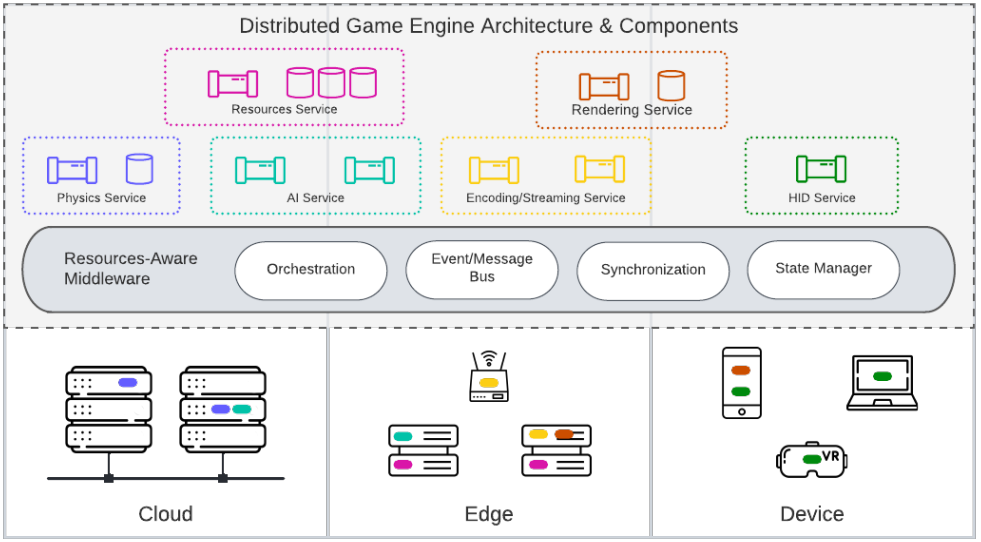
\includegraphics[width=1\linewidth]{immagini/State-of-the-art/resource-aware-middleware-architecture}
	\caption[Distributed architecture leaveraging a resource-aware middleware support.]{Distributed architecture leaveraging a resource-aware middleware support.}
	\label{fig:resource-aware-middleware-architecture}
\end{figure}
High priority was placed on the efficient management of virtual resources, implemented through a \textit{resource-aware support middleware}. This middleware exploits various techniques to abstract all aspects related to low-level management of edge-cloud resources, which are mainly composed of physical and virtual nodes with different computational, network and storage capabilities. \\
This is very relevant in the context of Game Engine modularization, since it ensures not only that the modules original functionalities are maintained, but also that the resources allocated for them actually meet their requirements. \\ \\
On a more technical level, the modules are implemented through Docker containers, which are both lightweight and interactive virtual environments, that fit well with the requirements of these distributed components. \\ \\
Overall this architecture proposes a very interesting approach to the modularization of Legacy Game Engines, especially with the introduction of the concept of Containerization, which provides the characteristics needed for a practical approach to system distribution. However, even if some performance tests have been conducted on the final architecture, there is still room for additional evaluations on the impact of network-related phenomenon (e.g. network latency and traffic) on the performance of such distributed systems.


\subsection{The impact of network latency on the User Experience}
As we saw in the previous sections Distributed Game Engines, regardless of the approach, need to work inside a network environment. Whether we decide to implement the distributed modules on Cloud virtual machines or on a local network, there is still a network layer that needs to be introduced into the picture, in order to allow these modules to communicate with each other. \\ \\
Often times researches do not include experiments related to the impact of network latency or traffic on the performance of their proposed architectures, as the focus is generally directed towards the actual performance of the system. \\
However, if we aim to provide a practical implementation of a Distributed Game Engine architecture, we cannot simply ignore the presence of these effects, which are present in realistic network environments. Moreover, the development of the distributed architecture itself should take these effects into account, when technical choices are made during the initial design. \\ \\
There have been studies, in fact, on the impact of network latency and game responsiveness on the players performance \cite{womak:framerate-player-FPS, womak:user-tolerance-latency, womak:player-latency-cloud}, particularly in the context of cloud-based games. The result is that, even with modest amounts of latency, the user performance can degrade up to 25\% with each 100 milliseconds of network latency, with a directly proportional general perception of QoE. Moreover, comparing these results for cloud-based games with traditional games, shows that they are as sensitive to latency as first person avatar games, which is the most sensitive class of games to latency. \\ \\
Network latency, however, does not impact the User Experience only through image delay. Legacy Game Engines are generally described as highly performant \cite{womak:revamping-cloud-games}, due to their monolithic nature that allows its different internal components to interact very efficiently between each other. \\ \\
On the other hand, in the context of Distributed Game Engines, the communication between the various modules can be slowed down or become unstable, due to problems in the network infrastructure. Considering role of the Game Engine modules in managing core functionalities of the software, it is to be expected for delays in their communications to also impact the actual performance of the system. For instance, if the module responsible for managing the graphics rendering of the game image is impacted by network latency, the graphics framerate is likely to become object of degradation, thus indirectly affecting the User Experience. \\ \\
Researches on the topic \cite{womak:framerate-player-FPS} have demonstrated how excessively low framerates have a very significant impact on the playability and QoE of the games. Moreover, gaming genres which require quick real-time reactions to the displayed image (e.g. FPS, racing games) are particularly sensible in this regard, thus the user tolerance is generally lower. \\ \\
As such, we can finally assert that the network infrastructure used for modules communication is a paramount aspect to consider when designing a Distributed Game Engine.

\subsection{Distributed systems' scalability}
In terms of scalability, Distributed Game Engines provide meaningful improvements, by allowing systems to not only scale vertically the quantity of available resources, but also horizontally through the offload of computational tasks to additional nodes or replicas. Still, this improvement comes also with some limits and drawbacks to consider. \\ \\
While Legacy Game Engine internal components are able to communicate directly with each other inside the same environment, this is different for Distributed Game Engine modules, which require an additional means to exchange data. This requirement is not necessarily a problem, since there are multiple ways to satisfy it, whether through socket-based communication between the modules or storage of data on shared memory. \\ \\ Nonetheless, as studies have shown \cite{womak:tame-efficient-task-allocation, womak:rafting-multiplayer-games, womak:distributed-minecraft}, the amount of remote calls that happen between the distributed modules is generally quite high and tends to generate a significant amount of workload for the means of communication. As the number of distributed modules increases, so does the amount of communication traffic introduced, since there are more components which require to have their remote calls carried out through the network. \\ \\
In this context, there are obviously limits to the amount of traffic a communication means can handle, whether because of network bandwidth constraints or finite amount of resources available for the shared memory. Reaching such limits can cause system congestion, and thus generate problematic phenomena, such as packet loss or network latency, that can undermine the performance of the whole distributed system. \\ \\
Considering this possibility, if we aim to effectively turn a Legacy Game Engine into a Distributed Game Engine, an evaluation needs to be conducted on which functions or components to actually offload into distributed modules \cite{womak:performance-analysis-game-engine}. The modularization of a needlessly large number of Game Engine functionalities could, in fact, pose us in this exact situation, whereas if too many of them are grouped inside the same modules, the benefits of a distributed approach could be significantly reduced. \\ \\
To sum up, it is important to strike a reasonable balance between the amount of modules in a Distributed Game Engine and the capabilities of the means of communication used to support them, considering the scalability limits present also in this kind of system.

\subsection{Synchronization of a shared game state}
The management of the game state has always been a problem even in classic client-server architectures \cite{womak:distributed-game-engine-android, womak:distributed-minecraft}. In such architecture, there is a constant exchange of information about the global state and the next player action, between the local client and the server. This process is generally managed as follows:
\begin{enumerate}
	\item the client receives a network message/packet, containing information about the current global state, often including data related to the specific client's player situation;
	\item the client computes the next action to be sent to the server, whether through Artificial Intelligence (AI) or through human input;
	\item the client sends the action to the server as a network message/packet, and the server proceeds to verify its validity with respect to the current game state;
	\item if the action is valid, the server computes the new global state and updates it, sending new information about it to the client;
	\item the process then repeats until the game is finished.
\end{enumerate}
While seemingly quite simple, this process becomes much harder to manage in the context of multiplayer gaming \cite{womak:rafting-multiplayer-games, womak:distributed-game-engine-android}, where the is more than one client interacting with the server and receiving game state updates. Moreover, in order to guarantee fairness to all players, it is important that they are all constantly provided with the same updated view of the game state.
\begin{figure}[h!]
	\centering
	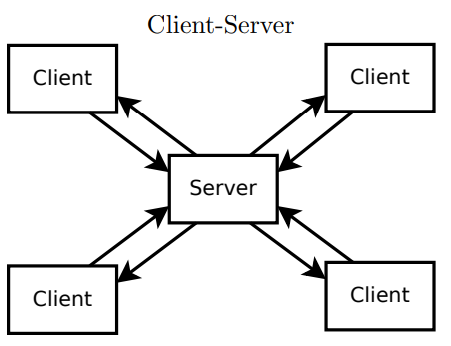
\includegraphics[width=0.55\linewidth]{immagini/State-of-the-art/simple-client-server}
	\caption[Simple view of a multi client-server architecture.]{Simple view of a multi client-server architecture.}
	\label{fig:simple-client-server}
\end{figure}
\\ With a monolithic architecture it is reasonable to identify the server as a single compact component, able to efficiently manage and update the game state. However, in the context of Distributed Game Engines this may not necessarily be the case, since the server itself is a distributed system with multiple components that need to interact with the game state.
\begin{figure}
	\centering
	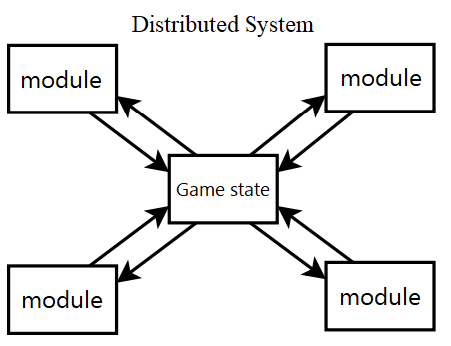
\includegraphics[width=0.55\linewidth]{immagini/State-of-the-art/simple-distributed-state}
	\caption[Simple view of a distributed system's state.]{Simple view of a distributed system's state.}
	\label{fig:simple-distributed-state}
\end{figure}
\\ \\The distributed modules require the same updated view of game state data, in order to correctly implement the original Game Engine functionalities, as well the possibility to modify such data concurrently with the other modules. This, however, is not a trivial task, since the management of consistent data can be hard without a dedicated infrastructure and, even in that context, the synchronization process can be computationally expensive for wide distributed systems or large amounts of data. Moreover, the actual storage of the game state is usually responsibility of a single component, which may incur in bottlenecks if the number of read/write requests is excessively high. \\ \\
For this reason, multiple researches \cite{womak:consistency-models-cloud-games, womak:distributed-minecraft, womak:distributed-game-engine-android} have studied how to make this process more efficient, with different approaches, such as:
\begin{itemize}
	\item usage of \textit{local independent game state}, with changes computed locally, and a \textit{remote game state} with which the local one is periodically synchronized \cite{womak:distributed-architecture-interactive-multiplayer}. This helps reducing the load on the game state management component, by reducing the frequency of updates;
	\item usage of \textit{multiple game state management components} \cite{womak:multiplayer-distributed-state}, with different characteristics, depending on the nature of the game state data to be stored. This could help distributing the traffic related to read/write requests among multiple components and providing the resources needed for processing different levels of workload;
	\item usage of \textit{Area of Interest (AoI)} \cite{womak:distributed-minecraft, womak:distributed-architecture-interactive-multiplayer}, for deciding which game state data should be requested to the storage component and which should be managed locally (cached).
\end{itemize}
The approaches to this problem may vary greatly, also in relation to the characteristics of the architecture that is being developed. \\
Still, considering the general performance requirements of Game Engines, we can understand how important it is to carefully consider how the distributed modules communication and game state data management are implemented in such systems.